\chapter{Goodbye Virtualenvs, Hello \texttt{guix shell}}
\label{chap:guix-shell}

\epigraph{``Docker: Because why solve dependency hell cleanly when you can just ship an entire Debian virtual machine for a 50-line Node.js script?''}{--- Modern DevOps proverb}

\noindent
Every software developer has experienced the nightmare of setting up a new development project:
\begin{enumerate}
  \item You clone the repository.
  \item The \texttt{README.md} tells you to install GCC 12, CMake 3.25, Python 3.10, PostgreSQL 14 client headers, and a very specific version of Rust.
  \item Your host operating system has GCC 14, Python 3.12, and CMake 3.20.
  \item You spend the next five hours fighting PPA repositories, Homebrew taps, and Docker permission issues.
\end{enumerate}

GNU Guix introduces the ultimate developer superpower: \guixcmd{guix shell}.

\section{The Concept: Disposable, Ephemeral Environments}

\guixcmd{guix shell} allows you to spawn a subshell containing any set of packages on demand, without polluting your user profile, without root permissions, and without touching your system's global files.

When you exit the subshell, the environment evaporates into thin air.

\begin{lstlisting}[style=guixcli]
# Spawn a shell with Python, Numpy, and GCC ready to go
guix shell python python-numpy gcc-toolchain

# Inside the shell, everything is configured:
[env]$ python3 -c "import numpy as np; print(np.__version__)"
1.23.2
[env]$ gcc --version
gcc (GCC) 11.3.0

# Exit the shell, and your host environment is completely untouched
[env]$ exit
$ which python3
/usr/bin/which: no python3 in ($PATH)
\end{lstlisting}

You can also run one-off commands directly without even dropping into an interactive prompt:

\begin{lstlisting}[style=guixcli]
# Run a one-liner inside a disposable Node.js environment
guix shell node -- node -e "console.log('Hello from Guix!')"
\end{lstlisting}

\section{Achieving True Isolation: \texttt{--pure}}

By default, \guixcmd{guix shell} merges the specified packages with your host environment variables (like your existing \texttt{\$PATH}). This is convenient for daily use, but what if you want to be 100\% sure your code doesn't accidentally depend on some random binary hidden in \texttt{/usr/local/bin}?

You add the \texttt{--pure} flag:

\begin{lstlisting}[style=guixcli]
guix shell --pure python python-requests -- python3 app.py
\end{lstlisting}

When \texttt{--pure} is specified, Guix clears almost all host environment variables. Only the packages explicitly declared on the command line exist in \texttt{\$PATH}.

\section{Containers Without Docker: The \texttt{-C} Flag}

Now for the real magic. Guix contains a built-in container engine based on unprivileged Linux kernel namespaces (mount, PID, network, IPC, and UTS namespaces).

By passing the \texttt{-C} (or \texttt{--container}) flag, Guix creates a lightweight, isolated Linux container on the fly:

\begin{lstlisting}[style=guixcli]
guix shell --container python bash coreutils
\end{lstlisting}

Inside this container:
\begin{itemize}
  \item The filesystem contains \textbf{only} \texttt{/gnu/store} and an empty \texttt{/tmp}.
  \item Your real \texttt{/home} directory is completely invisible.
  \item The process cannot see or kill any processes running on the host system.
  \item Network access is disabled by default!
  \item You did \textbf{NOT} need \texttt{sudo}, a root daemon, or a Docker service running in the background.
\end{itemize}

\begin{tearsbox}[Docker Daemon vs Guix Container]
Docker requires a root-privileged daemon listening on a Unix socket, custom overlay filesystems, non-reproducible \texttt{Dockerfile} scripts that run \texttt{curl ... | bash}, and layers upon layers of cached bloat.

\guixcmd{guix shell -C} uses native Linux kernel namespaces directly, boots in 50 milliseconds, shares the immutable \texttt{/gnu/store} directly with zero copy-on-write overhead, and is completely unprivileged.
\end{tearsbox}

\begin{figure}[htbp]
\centering
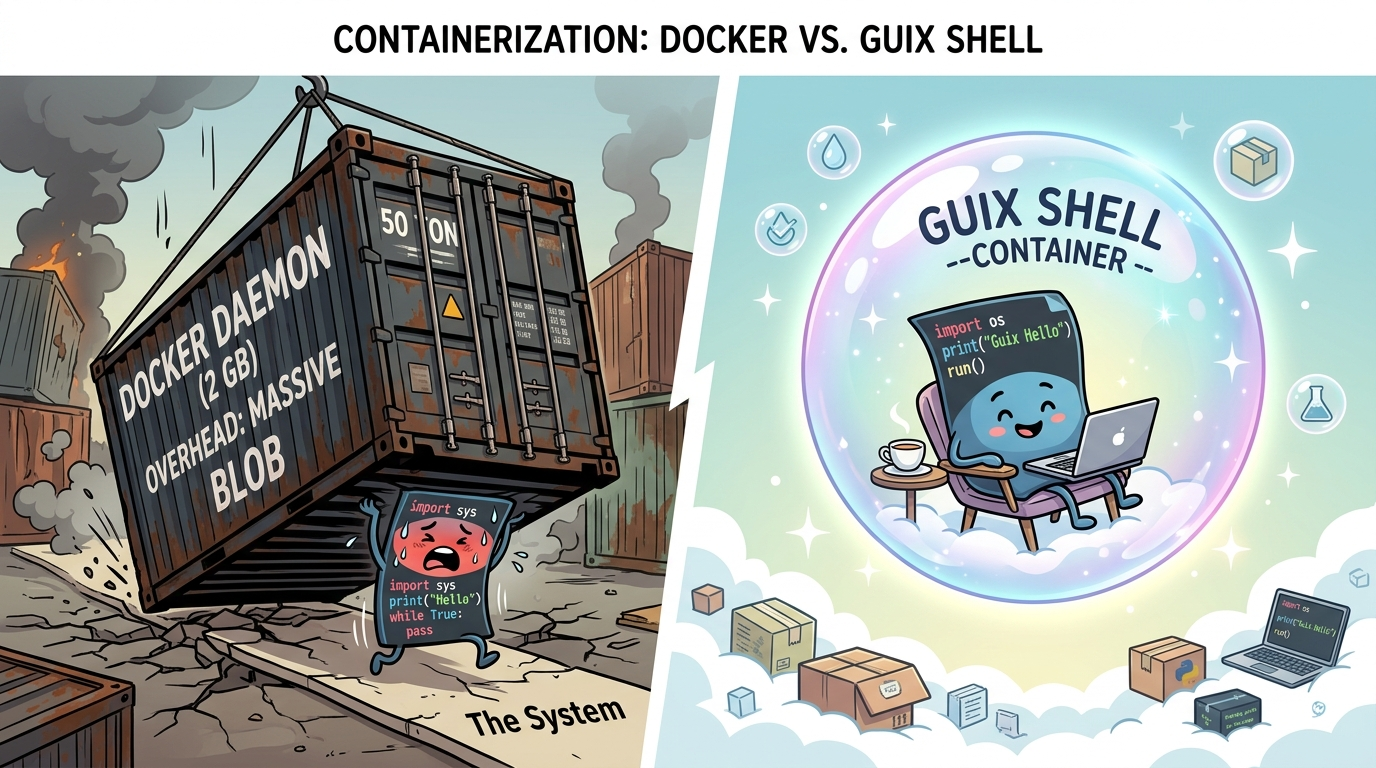
\includegraphics[width=0.92\textwidth]{images/docker_vs_guix_shell.jpg}
\caption*{\textit{Figure 4.1: Containerization contrast: 50 tons of root-privileged Docker overhead crushing a 3-line script versus the weightless, unprivileged bubble of \guixcmd{guix shell --container}.}}
\end{figure}

\section{Fine-Grained Sharing: Filesystems and Network}

What if your containerized application needs access to a local dataset or needs to make HTTP requests? Guix provides granular flags:

\begin{lstlisting}[style=guixcli]
guix shell --container \
  --network \
  --expose=/data/images=/mnt/images:ro \
  --share=/home/user/workspace=/app \
  python python-torch \
  -- python3 /app/train.py
\end{lstlisting}

Let us break down these flags:
\begin{itemize}
  \item \guixcmd{--network} (or \guixcmd{-N}): Grants network namespace access (enables outbound/inbound internet).
  \item \guixcmd{--expose=HOST=GUEST:ro}: Mounts a host directory inside the container as \textbf{read-only}.
  \item \guixcmd{--share=HOST=GUEST}: Mounts a host directory inside the container with \textbf{read-write} permissions.
\end{itemize}

\section{The Instant Development Environment: \texttt{-D}}

Suppose you want to contribute to an existing open-source package packaged in Guix, such as \texttt{inkscape}, \texttt{curl}, or \texttt{qemu}. 

How do you get all of its 50+ build dependencies, header files, libraries, and compilers set up on your machine?

\begin{lstlisting}[style=guixcli]
# Enter a shell with all build dependencies of Inkscape installed!
guix shell -D inkscape
\end{lstlisting}

The \texttt{-D} (or \texttt{--development}) flag inspects the Guix package recipe for \texttt{inkscape}, gathers all of its \texttt{inputs}, \texttt{native-inputs}, and \texttt{propagated-inputs}, and drops you into a shell where every single build dependency is available. You can immediately run \texttt{cmake} and \texttt{make} without installing a single package globally!

\begin{protipbox}[The Development Flag on Local Recipes]
You can even use \texttt{-D -f guix.scm} to load the development environment defined in your own project's local package file! We will explore this in Chapter~\ref{chap:manifests}.
\end{protipbox}
